% Тут используется класс, установленный на сервере Papeeria. На случай, если
% текст понадобится редактировать где-то в другом месте, рядом лежит файл matmex-diploma-custom.cls
% который в момент своего создания был идентичен классу, установленному на сервере.
% Для того, чтобы им воспользоваться, замените matmex-diploma на matmex-diploma-custom
% Если вы работаете исключительно в Papeeria то мы настоятельно рекомендуем пользоваться
% классом matmex-diploma, поскольку он будет автоматически обновляться по мере внесения корректив
%
\documentclass{matmex-diploma-custom}

\usepackage{amsfonts}
\usepackage{amsmath}
\usepackage{hyperref}

\usepackage{listings}
\lstset{language=Java, captionpos=b, basicstyle=\footnotesize, breakatwhitespace=true, breaklines=true}
\renewcommand{\lstlistingname}{Код программы}



\begin{document}
\filltitle{ru}{
    chair              = {Кафедра Информатики},
    title              = {Анализ возможности и эффективности параллельной реализации алгоритма packJPG},
    type               = {diploma},
    position           = {студента},
    group              = 461,
    author             = {Шмагринский Игорь Олегович},
    supervisorPosition = {к.\,ф.-м.\,н., доцент},
    supervisor         = {{\sigplace{Н.Ю.~Ловягин}{подпись}}},
    reviewerPosition   = {д.\,ф.-м.\,н., ассистент},
    reviewer           = {{\sigplace{Н.Н.~Неизвестный}{подпись}}},
    chairHeadPosition  = {д.\,ф.-м.\,н., профессор},
    chairHead          = {{\sigplace{В.О.~Костин}{подпись}}},
%   university         = {Санкт-Петербургский Государственный Университет},
%   faculty            = {Математико-механический факультет},
%   city               = {Санкт-Петербург},
%   year               = {2013}
}
\filltitle{en}{
    chair              = {Chair of Computer Science},
    title              = {Analysis of the possibility and efficiency of the parallel implementation of the packJPG algorithm},
    author             = {Igor Shmagrinsky},
    supervisorPosition = {docent},
    supervisor         = {{\sigplace{N.Y.~Lovyagin}{signature}}},
    reviewerPosition   = {professor},
    reviewer           = {{\sigplace{N.N.~Neizvestny}{signature}}},
    chairHeadPosition  = {professor},
    chairHead          = {{\sigplace{V.O~Kostin}{signature}}},
}
\maketitle
\tableofcontents
\newpage
% У введения нет номера главы
\section*{Введение}

    IT технологии не стоят на  месте и развиваются с неимоверной скоростью, сейчас трудно представить, что когда-то в большинстве устройств был всего лишь один процессор. Сейчас даже в мобильных аппаратах присутствует более чем одно вычислительное устройство. Это позволяет выполнять трудоемкие операции в несколько раз быстрее,но многие в наше время забывают об адаптации алгоритмов для многопроцессорных аритектур, поэтому большинство программ работают неэффективно и использую не всю мощь современных устройств.

 В данной работе расмотрен один из эффективнейших алгоритмов сжатия изображения PackJPG, который уступает другим алгоритмам своей области лишь по времени работы. В ходе исследования будет проведено исследование возможности адаптации данного алгоритма и его реализация на для многоядерных процессоров с помощью технологи OpenCL. Так же будет выполненма оценка времени работы алгоритма, его реальное время и сравнение трудоемкости существующих алгоритмов сжатия изображений и  нашей реализации.

\section{Предварительные сведения}
Сжатие это техника направленная на понижение размерности данных без  чрезмерной потери качества мультимедийных данных.
Перемещение и хранение сжатых мультимединых  файлов намного быстрее  и эффективнее, чем у оригинальных данных. Если при сжатии уменьщается снижается качество исходных данных то это сжатие с потерями, иначе - без потерь. Существует множестнво разнообразных  техник и стандартов для сжатия мультемедийных данных с потерями, одним из таких стандартов протяжении многих лет является формат изображений JPEG.
\subsection{Стандарт сжатия изображений JPEG}
JPEG-это стандарт сжатия изображений разработаный Joint Photogrphic Experts Group. Он был официально одобрен мировым сообществом в 1992 году. JPEG содержит некоторое число шагов, каждый из которых способствует процессу сжатия.
Рассмотрим каждый из них детально.
\subsubsection{Кодирование}
Хотя \emph{JPEG} файл может закодирован разными путями, но самый известный и популярный - \emph{JFIF} кодировние.
Процесс кодирования сстоит из нескольких шагов.\\

\textbf{Преобразование цветового пространства} \newline

Многие цвета изображения представлены с помощью цветового пространства \emph{RGB}. Такое представление, однако, сильно коррелирует, что подразумевает, что это цветовое пространство не очень подходит для независимого кодирования. Так как человеческая зрительная система менее чувствительна к позиции и движению ярких  цветов. \\
Следовательно, целесообразней изпользовать цветовое пространство \emph{YCrBr}.\\

\textbf{Разбиение исходного изображения}\newline

После изображение разбивается yа блоки 8x8 пикселей, с каждым из которых ведется дальнейшая работа.\\

\textbf{Дискретное косинусное преобразование}\newline

Дальше каждая компонента \emph{(Y,Cr,Br)} каждого блока преобразуеется к  частотной форме. Для  этого используется двумерное диоскретное косинусное преобразование второго типа. Перед вычислением этого преобразования, все значения сдвигаются из положительного интервала $[0,255]$в интервал $[-128, 127]$ вычитеанием из каждой значения компоненты блока 128. Это действие является обязательным, так такой интервал значений является одним из требований для дискретного косинусного преобразования. В резултате будет полуен блок $g_{x,y}$ с которым мы будем работать дальше.\newline

Блок $ g $ преообразуется по следующему принципу:
$$ \ G_{u,v} =
    \frac{1}{4}
    \alpha(u)
    \alpha(v)
    \sum_{x=0}^7
    \sum_{y=0}^7
    g_{x,y}
    \cos \left[\frac{(2x+1)u\pi}{16} \right]
    \cos \left[\frac{(2y+1)v\pi}{16} \right],
  $$
  где:
  \begin{itemize}
  \item{$u$ - вертикальная пространственная частота для целых чисел $\ 0 \leq u < 8$}
  \item{$v$ - горизонатальная пространственная частота для целых чисел $\ 0 \leq v < 8$}
  \item{
    $\alpha(u) =
    \begin{cases}
        \frac{1}{\sqrt{2}}, & \mbox{if }u=0 \\1, & \mbox{иначе}
    \end{cases}$
    - норма необходимая  для того чтобы преобразование было ортомнормированным.
  }
  \item{
    $\ g_{x,y}$ - это значение которое содержит в себе пиксель с координатами $\ (x,y)$
  }
    $\ G_{u,v}$ - это значение которое содержит в себе пиксель с координатами $\ (u,v)$
  }
  \end{itemize}

  После преобразования можно заметить что значение $ G_{0,0} $  превосходит все остальные, его так же называют
  \emph{коэффициентом DC}. Он определяет основной тон для блока в целом. Его так же можно назвать
  \emph{постоянной компонентой}. Оставшиеся 63 коэффициента (блока 8x8) называют \emph{AC
  коэффициентами}, где AC могут быть установлены для запасных комп                                                  онент.
  % TODO: уточнить про AC коэфициенты % 2dd `2
  Преимущество дискретного косинусного преобразования - возможность вычислить основной оттенок блока (сигнала).\\

\textbf{Квантование}\newline

Человеческий глаз  хорошо приспособлен замечать маленькие различия в яркости на относительно больших расстояниях, но плохо отличает точную силу яркости на высоких частотах. Это позволяет значительно уменьшить количество информации о высокого частотных компонентах. Данную операцию можно  осуществить простым делением значения  каждой компоненты в частотном диапозоне на константу и последующим округлением этого значения ближайшим целым числом. Это действие, единственное во всем процессе сжатия при котором происходит потеря данных, в отличии от дискретного косинусного пребразования, которое выполняет вычисления с выской точностью. Как результат, многие компоненты оказваются равны  нулю или их значение очень близко к нулю, как следствие они занимают меньше бит в памяти.

%The human eye is good at seeing small differences in brightness over a relatively large area, but not so good at distinguishing the exact strength of a high frequency brightness variation. This allows one to greatly reduce the amount of information in the high frequency components. This is done by simply dividing each component in the frequency domain by a constant for that component, and then rounding to the nearest integer. This rounding operation is the only lossy operation in the whole process (other than chroma subsampling) if the DCT computation is performed with sufficiently high precision. As a result of this, it is typically the case that many of the higher frequency components are rounded to zero, and many of the rest become small positive or negative numbers, which take many fewer bits to represent.
Подобные процессы, когда процедура построения чего-либо ведтся с помощью набора дискретных (в нашем случае целых) велечин называется \emph{квантованием}.

Элементы \emph{матрицы квантования} управляют коэфициентом сжатия. Чем больше значение компонент, тем больше будет потеря изображения в качетсве. Типичная матрица квантования (качество ухудшается примерено на 50\%, утверждена как часть стандарта JPEG), выглядит следующим образом:
%The elements in the quantization matrix control the compression ratio, with larger values producing greater compression. A typical quantization matrix (for a quality of 50% as specified in the original JPEG Standard), is as follows:
$$ Q=
     \begin{bmatrix}
      16 & 11 & 10 & 16 & 24 & 40 & 51 & 61 \\
      12 & 12 & 14 & 19 & 26 & 58 & 60 & 55 \\
      14 & 13 & 16 & 24 & 40 & 57 & 69 & 56 \\
      14 & 17 & 22 & 29 & 51 & 87 & 80 & 62 \\
      18 & 22 & 37 & 56 & 68 & 109 & 103 & 77 \\
      24 & 35 & 55 & 64 & 81 & 104 & 113 & 92 \\
      49 & 64 & 78 & 87 & 103 & 121 & 120 & 101 \\
      72 & 92 & 95 & 98 & 112 & 100 & 103 & 99
     \end{bmatrix}.
$$

Квантование коэффициентов матрицы  G, полученной на предыдущем шаге, происходит следующим образом:
% The quantized DCT coefficients are computed with
е
$$B_{j,k} = \mathrm{round} \left( \frac{G_{j,k}}{Q_{j,k}} \right) \mbox{ для } j=0,1,2,\ldots,7; k=0,1,2,\ldots,7$$

 % B_{j,k} = \mathrm{round} \left( \frac{G_{j,k}}{Q_{j,k}} \right) \mbox{ for } j=0,1,2,\ldots,7; k=0,1,2,\ldots,7

  %where G is the unquantized DCT coefficients; Q is the quantization matrix above; and B is the quantized DCT coefficients.
  Полученная матрица B, отправляется на следующий шаг, где будет произвоидиться ее энтропийное кодирование.\\
  %Using this quantization matrix with the DCT coefficient matrix from above results in:

\textbf{Энтропийное кодирование}\\

\emph{Энтропийное кодирование} - это специальная форма сжатия данных без потерь. Она включает в себя переобределение порядка компонент изображения в виде \emph{"зиг-зага"} (рис. 1) дальнейшее сжаатие методом \emph{кодирования повторов}, который группирует похожие повторяющие значения вместе. Затем к получивишейся последовательности применяется \emph{Код Хаффмана}.\\

    \begin{figure}
      \centering
        \reflectbox{%
          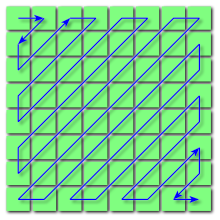
\includegraphics[width=0.5\textwidth]{images/zig-zag.png}}
      \caption{Порядок "зиг-заг" в котором кодируются компонеты блока.}
      % TODO: сделать  ссылки на изображения
    \end{figure}
 %Entropy coding is a special form of lossless data compression. It involves arranging the image components in a "zigzag" order employing run-length encoding (RLE) algorithm that groups similar frequencies together, inserting length coding zeros, and then using Huffman coding on what is left.
% TODO: Перести этот абзац.
 %  The previous quantized DC coefficient is used to predict the current quantized DC coefficient. The difference between the two is encoded rather than the actual value. The encoding of the 63 quantized AC coefficients does not use such prediction differencing.

Рассмотрим процесс кодирования данных уже представленных в "зиг-заг" порядке, начиная c объяснения, что такое кодирование повторов, дадим некоторые определения :

 %The process of encoding the zig-zag quantized data begins with a run-length encoding explained below, where:

\begin{itemize}
    \item{
        $x$ - ненулевой, AC коэфициент получившийся после квантования.
    }
    %x is the non-zero, quantized AC coefficient.
    \item{
        $RUNLENGTH$ - число нулей которые следуют перед ненулевым AC коэффициентом
    }
     %RUNLENGTH is the number of zeroes that came before this non-zero AC coefficient.
     \item{
        $SIZE$ - число бит требуемых, чтобы представить $x$.
     }
      %SIZE is the number of bits required to represent x.
    \item{
        $AMPLITUDE$ - побитовое представление $x$.
    }
     %AMPLITUDE is the bit-representation of x.
\end{itemize}

Кодирование повторов работает исследуя каждый  ненулевой AC коэффицинт x и определяя, как много нулей следует перед ним. C этой иноформацией и создаются два \emph{символа}.

 %The run-length encoding works by examining each non-zero AC coefficient x and determining how many zeroes came before the previous AC coefficient. With this information, two symbols are created:

  $$ \begin{bmatrix}
        Symbol 1 & Symbol 2 \\
        RUNLENGTH, SIZE& AMPLITUDE\\

       \end{bmatrix}. $$\\

  Оба числа RUNLENGTH и SIZE  хранятся в одном и том же байте, под каждый из них отводится по 4 бита. Так значения любого из них не превосходит 64.

 %Both RUNLENGTH and SIZE rest on the same byte, meaning that each only contains four bits of information. The higher bits deal with the number of zeroes, while the lower bits denote the number of bits necessary to encode the value of x.

Так же в стандарте определены специальные символы, которые означают окочание блока \emph{EOB}, и еще один на случай когда встречаются более более 15 нулей подряд, до достижения ненулевого коэффицинта, тогда символ кодируется специально как: (15, 0) (0).
 %This has the immediate implication of Symbol 1 being only able store information regarding the first 15 zeroes preceding the non-zero AC coefficient. However, JPEG defines two special Huffman code words. One is for ending the sequence prematurely when the remaining coefficients are zero (called "End-of-Block" or "EOB"), and another when the run of zeroes goes beyond 15 before reaching a non-zero AC coefficient. In such a case where 16 zeroes are encountered before a given non-zero AC coefficient, Symbol 1 is encoded "specially" as: (15, 0)(0).

 Весь процесс продолжается до тех пор пока не будет достигнут сивол окончания блока. Определенный как символ  EOB - (0,0).\\

 %The overall process continues until "EOB" – denoted by (0, 0) – is reached.

 %With this in mind, the sequence from earlier becomes:

\subsubsection{Декодирование}

Декодирование для отображения изображения состоит из тех же шагов, выполняемых в обратном порядке.

%Decoding to display the image consists of doing all the above in reverse.

Возьмем раскодированую матрицу коэффициентов, полученную после примения к ней дешифрования кода Хаффмана и декодирование повторов. И расположим символы этой последовательности в правильном порядке. В результате получится матрица $B$, являющуюся результатом шага квантования.
%Taking the DCT coefficient matrix (after adding the difference of the DC coefficient back in)
После умножим матрицe $B$  на матрицу квантования $Q$ по Адамару. В результате получим матрицу $F$

%and taking the entry-for-entry product with the quantization matrix from above results in
$$ F = B \circ Q $$

которая очень похожа на оригинальную  матрицу $G$, явяляющуюся результатом дискретного косинусного преобразования.

%which closely resembles the original DCT coefficient matrix for the top-left portion.

Следующим шагом является применение обратного косинусного преобразования, которое можно описать слкдюущим образом:

%The next step is to take the two-dimensional inverse DCT (a 2D type-III DCT), which is given by:

$$f_{x,y} =
 \frac{1}{4}
 \sum_{u=0}^7
 \sum_{v=0}^7
 \alpha(u) \alpha(v) F_{u,v}
 \cos \left[\frac{(2x+1)u\pi}{16} \right]
 \cos \left[\frac{(2y+1)v\pi}{16} \right]

$$
%where

где

\begin{itemize}
\item{
$\ x$ столбец пикселей $\ 0 \leq x < 8$.
}
\item{
$\ y$ строка пикселей $\ 0 \leq y < 8$.
}
\item{
$\ F_{u,v}$ это компонента матрицы коэффициентов полученая на предыдущем шаге с координатам $\ (u,v)$.
}
\item{
$\ f_{x,y}$ - значение полученой компоненты с координатами $\ (x,y)$
}
\end{itemize}

После значения  каждой компоненты округляются до ближеайшего целого числа, так изначально значение компоненты целочисленное, и к каждому значению прибавляется 128. На этом процедура декодирования заканчивается. И мы получаем изображени практически идентичное оригиналу.
%Rounding the output to integer values (since the original had integer values) results in an image with values (still shifted down by 128)



%Notice the slight differences between the original (top) and decompressed image (bottom), which is most readily seen in the bottom-left corner.

%and adding 128 to each entry

%This is the decompressed subimage. In general, the decompression process may produce values outside the original input range of [0, 255]. If this occurs, the decoder needs to clip the output values keep them within that range to prevent overflow when storing the decompressed image with the original bit depth.

%The decompressed subimage can be compared to the original subimage (also see images to the right) by taking the difference (original − uncompressed) results in the following error values:


%with an average absolute error of about 5 values per pixels (i.e., \frac{1}{64} \sum_{x=0}^7 \sum_{y=0}^7 |e(x,y)| = 4.9197).

%The error is most noticeable in the bottom-left corner where the bottom-left pixel becomes darker than the pixel to its immediate right.
\subsubsection{Представление}
\subsection{Сжатие JPEG изображений без потерь}
\subsection{Технология OpenCL}
\section{Алгоритм packJPG}

PackJPG это пограмма специально разработанная для дальнейшего сжатия JPEG изображений без потерь. Обычно ей удается уменьшить размер файла JPEG изображения  примерно на 20\%.
% packJPG is a compression program specially designed for further compression of JPEG images without causing any further loss. Typically it reduces the file size of a JPEG file by 20%.

Основной идея алгоритма сжатия в этой программе такова, что сначла JPEG изображение декодируется до шага квантования коэффициентов дискретного косинусного преобразования. Каждый блок 8х8 содержит по 64 цветовые компоненты. Представим, что изображение разбито на эти блоки, мы берем из каждого блока компоненты с координатами $(x,y)$, и групируем их в одно новое \emph{подизображение}. Далее к получившейся последвателности компомнент применятся сразу несколько алгоритмов сжатия, каждый из которых будет рассмотрен подробнее.

  \subsection{Предиктивное кодирование}
  Сгруппированные коэфициенты демонстрируют нам уменьшенную версию оригинального изображения. Следовательно к сгруппированным подизображениям можно применить технику \emph{предиктивного кодирования}.


\subsection{Основная идея}
\subsection{Коды Хаффмена}
\subsection{Арифмитическое кодирование}
\section{Анализ возможности реализации с помощью технологии OpenMP}
\section{Результаты}

% У заключения нет номера главы
\section*{Заключение}

\bibliographystyle{ugost2008}
\bibliography{diploma.bib}
\end{document}